\documentclass{article}
\usepackage[utf8]{inputenc}
\usepackage{graphicx}
\usepackage{float}

\title{Resultados de la Tarea 3 de Metodos Computacionales}
\author{Juan Felipe Cabrera 201530946}
\date{Julio 2017}
\begin{document}
\maketitle
\pagenumbering{arabic}

\section{Introducción}
El presente documento presenta lo resultados de la tercera tarea del curso de Metodos Computacionales.
\section{Punto 1: Onda}
Los resultados de este punto son dos imágenes que muestran los estados de la cubeta en los tiempos 30 y 60.
\subsection{Tiempo 30}
En el tiempo 30 se muestran los primeros rebotes de las ondas en las paredes.
\begin{figure}[H]
\centering
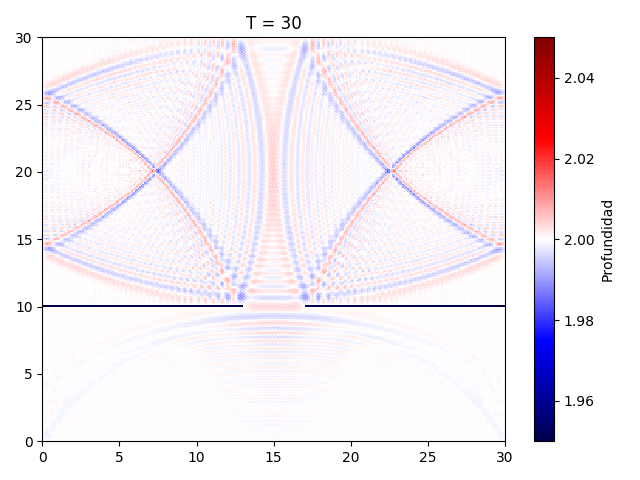
\includegraphics[scale=0.5]{30.png}
\caption{Tiempo 30}
\end{figure}
\newpage
\subsection{Tiempo 60}
En el tiempo 60 se ve algo de caos que resulta de varios rebotes y superposiciones de las ondas.
\begin{figure}[H]
\centering
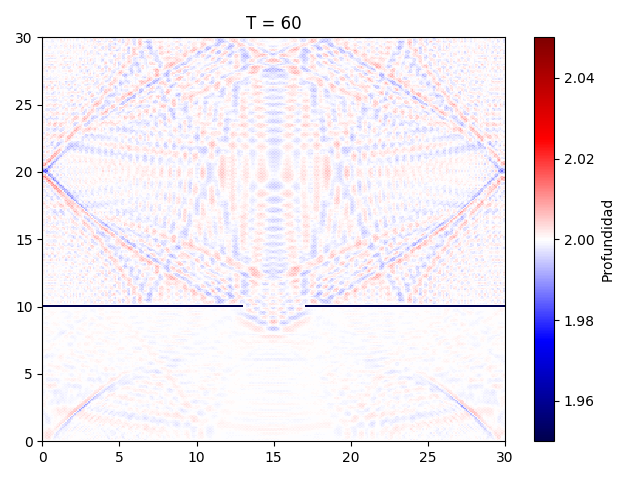
\includegraphics[scale=0.5]{60.png}
\caption{Tiempo 60}
\end{figure}
\section{Punto 2: Planetas}
El resultado de este punto es una gráfica de las orbitas de los planetas del sistema solar. Para contruirla se simularon 250 años equivalentes a aproximadamente el periodo de rotación de Plutón.
\begin{figure}[H]
\centering
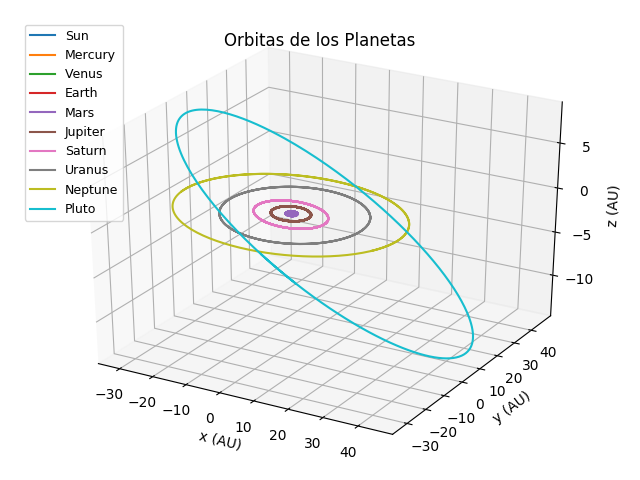
\includegraphics[scale=0.5]{orbitas.png}
\caption{Orbitas}
\end{figure}

\end{document}

